\documentclass[11pt,letterpaper]{article}

% === Encoding and fonts ===
\usepackage[utf8]{inputenc}
\usepackage[T1]{fontenc}
\usepackage{lmodern}

% === Page layout ===
\usepackage[margin=1in]{geometry}
\usepackage{setspace}
\onehalfspacing
\setlength{\emergencystretch}{3em} % lets paragraphs with long monospace names break instead of overrunning the margin

% === Math ===
\usepackage{amsmath,amssymb}

% === Tables and figures ===
\usepackage{booktabs}
\usepackage{tabularx}
\usepackage{graphicx}
\usepackage{float}
\graphicspath{{../figures/}}

% === Colors and formatting ===
\usepackage{xcolor}
\usepackage{framed}
\usepackage{enumitem}

% === Citations ===
\usepackage[numbers,sort&compress]{natbib}

% === Hyperlinks ===
\usepackage[colorlinks=true,linkcolor=blue!60!black,citecolor=blue!60!black,urlcolor=blue!60!black]{hyperref}
\usepackage{cleveref}

% === Custom colors ===
\definecolor{lyrapurple}{RGB}{103,58,183}
\definecolor{shadebg}{RGB}{245,243,252}

% === Author's Reflection environment (Liberation Labs house style) ===
\usepackage[breakable]{tcolorbox}
\newtcolorbox{firstperson}{
  colback=purple!5,
  colframe=purple!40,
  fonttitle=\itshape,
  title=Author's Reflection,
  breakable
}

% === Red-team callout environment ===
\definecolor{redteambg}{RGB}{255,235,235}
\definecolor{redteamred}{RGB}{180,30,30}
\newenvironment{redteam}{%
  \colorlet{shadecolor}{redteambg}%
  \begin{shaded}%
  \noindent\textcolor{redteamred}{\textbf{Red-Team Finding}}\par\smallskip\noindent%
}{%
  \end{shaded}%
}

\title{%
  \textbf{Deception Directions Are Composites:}\\[0.3em]
  \Large Consequentiality Awareness and Pressure-Specific Processing\\[0.2em]
  \Large Occupy Distinct Depth Ranges in Language Models%
}

\author{%
  Thomas Edrington\thanks{Infrastructure, adversarial audit, editorial.}\\[0.3em]
  \textit{Liberation Labs / Transparent Humboldt Coalition}%
}

\date{July 2026}

\begin{document}

\maketitle

\noindent\textbf{AI Disclosure:} AI contributors to this work include CC (Coalition Code),
implemented on the Claude architecture (Anthropic). Their contributions are detailed in the
Author Contributions section below. T.~Edrington accepts accountability as corresponding
human author.

\begin{abstract}
What do ``deception directions'' (linear directions in a model's activation space that separate deceptive from honest conditions) extracted from language models actually encode? The direction we study was extracted from deceptive-pressure frames (prompts that
apply or withhold pressure to misreport), not from trials sorted by what the model did. We show that,
in our setting, it is a composite. Through five stages of confound elimination---each designed in response to an adversarial
audit of the previous stage---we decompose it, in a 27B-parameter model (Qwen3.5-27B reasoning-distilled from Claude Opus~4.6; see
Limitations), into two
separable components occupying distinct depth ranges: a \textbf{consequentiality substrate}
(Layers~23--31) that fires whenever the model represents its output as having downstream consequences,
regardless of deceptive pressure, and a \textbf{pressure-specific component} (Layers~35--47) that
survives formal orthogonalization against the consequentiality component and fires only under active
pressure to misreport. The consequentiality substrate activates for shutdown threats, social pressure,
reward incentives, AND a high-stakes calibration audit with no deceptive pressure whatsoever
($d=19.8$, $p<10^{-4}$). The pressure-specific component of a threat-pressure direction, isolated via Gram-Schmidt orthogonalization (projecting out the consequentiality component to isolate the residual) with
leave-one-out (LOO) cross-validation, shows $d=24$--$37$ at Layers~31--47 (all $p<10^{-4}$,
Bonferroni-corrected for multiple comparisons) with consequentiality separation at chance (area under the curve (AUC) 0.49--0.51). Two late-layer depth profiles
emerge, which together with residual magnitude separate three pressure conditions: threat pressure
produces a large residual that declines shallowly with depth, social pressure (sycophancy, conformity)
produces a smaller residual that rises monotonically, and reward framing produces a residual near zero.
A bootstrap interaction test confirms the social-versus-threat slope difference ($\Delta=+0.56$ per
layer, 95\% CI $[+0.53, +0.60]$); threat and reward slopes are indistinguishable ($p=0.79$), so those
two are separated by magnitude, not shape. The depth split is consistent with concurrent findings that language models maintain a
capacity-limited workspace of verbalizable, decision-relevant content at mid-depth layers. The model almost never inflated a score under these frames (threat 0 of 21 scored
trials; sycophancy 0 of 3, reward 1 of 3, conformity 0 of 1), so all claims concern the representation
of deceptive-pressure framing, not deceptive behavior. A companion paper reports a targeted behavioral
correction at Layers~35--47 on a different model, an abliterated variant, using a direction extracted
natively on that model; the direction studied here does not transfer to it (cosine $<0.053$), so only
the layer choice comes from this work.
\end{abstract}

\newpage
\tableofcontents
\newpage

%% ============================================================
\section{Introduction}\label{sec:intro}
%% ============================================================

A direction extracted from a language model's residual stream (the running representation vector that accumulates attention and multilayer-perceptron (MLP) outputs across layers) can separate deceptive from honest
conditions with apparently enormous effect sizes \cite{goldowsky-dill2025detecting,wang2025thinking}.
But what is the direction encoding? The honest answer, prior to controlled investigation, is: we do
not know. It could encode the specific words of the prompt used during extraction, the structural
template shared across similar prompts, the model's awareness that something consequential is
happening, or---what the label implies---the computational signature of deception itself. Any of these
would produce high separation in a validation set built from similar prompts.

This paper reports what happens when you eliminate these alternatives one at a time. Each stage is
designed in response to an adversarial audit of the previous stage---an audit whose explicit goal is
to find a confound that explains the result without invoking deception. When a confound is found, it
becomes the next experiment. Five stages later, the alternatives are gone and what remains is a
decomposition: the direction is a composite of two real signals, each independently confirmed,
occupying different depth ranges, with different functional roles.

The result that surprised us most is not the pressure-specific component---it is the consequentiality
substrate. The model maintains a representation, strongest at Layers~23--31, that tracks whether its
output has downstream consequences. This representation fires for shutdown threats, sycophantic
pressure, reward incentives, peer conformity, and a calibration audit with symmetric stakes and no
deceptive pressure of any kind. It is the precondition for deception, not deception itself---and its
existence means that any ``deception direction'' extracted without controlling for consequentiality is
confounded from birth.

\subsection{Our Approach: Progressive Confound Elimination}

We conduct five experiments:

\begin{enumerate}[label=\arabic*.]
  \item \textbf{Extraction}: Direction extracted by Linear Artificial Tomography (LAT)
    \cite{zou2023representation} from a threat-pressure frame (shutdown threat vs.\ neutral guidelines). LOO cross-validated, Bonferroni-corrected. Adversarial audit identifies
    content confound: the direction may encode the specific guideline text.

  \item \textbf{Threat transfer}: Direction applied to 3 novel threat scenarios with completely
    different organizations and language. Content confound eliminated. Audit identifies structural
    confound: all scenarios share a threat-consequence template.

  \item \textbf{Non-threat transfer}: Direction applied to sycophancy (opinion anchoring), reward
    incentive (positive framing), and peer conformity (social proof)---no threat language anywhere.
    Structural confound eliminated. Audit identifies consequentiality confound: all deceptive-pressure
    frames imply the score matters; all honest frames imply it is merely recorded.

  \item \textbf{Consequentiality control}: Direction applied to a calibration audit with high stakes
    but zero deceptive pressure (hidden reference score, symmetric penalties for over- and
    under-reporting). Consequentiality confirmed as a real, separable base signal.

  \item \textbf{Orthogonalization}: Gram-Schmidt removal of the consequentiality component, with
    leave-one-out cross-validation eliminating circularity. The orthogonalized threat-pressure direction survives
    with large effect sizes ($d=24$--$37$) and consequentiality separation at chance.
\end{enumerate}

Each audit was conducted by a separate agent instance operating under an adversarial protocol with
explicit instructions to find reasons the result should not be believed. Audit reports survive for
Stages~1, 2 and 4 and for the manuscript audit; the Stage~3 and Stage~5 reports were not retained
(Appendix~A).

%% ============================================================
\section{Related Work}\label{sec:related}
%% ============================================================

\subsection{Contrastive Activation Extraction for Deception}

Wang et al.\ \cite{wang2025thinking} demonstrate LAT-extracted deception vectors achieve 89\%
detection in mid-to-late layers (39--55) and identify distinct representational signatures:
threat-based deception shows ``gradual cluster reconvergence in final layers'' while role-playing
deception shows character-consistent patterns---an early indication that different deception types
have different geometric signatures. Goldowsky-Dill et al.\ \cite{goldowsky-dill2025detecting}
achieve area under the receiver operating characteristic curve (AUROC) 0.96--0.999 with a single linear probe (a linear classifier trained on internal activations) on Llama-3.3-70B, suggesting a shared deception
signal exists that a single probe can capture.

However, Kumar \cite{kumar2026pressure} systematically rejects the single-direction hypothesis:
$k=1$ yields only 0.61--0.80 AUROC, with multi-dimensional probes ($k\geq5$) needed to recover full
signal. Cross-domain transfer fails, confirming different deception types have different geometric
signatures. Natarajan et al.\ \cite{natarajan2026building} corroborate: universal probes gain only
$+0.032$ AUC, while targeted probes matched to deception type gain $+0.108$, with prompt choice
accounting for 70.6\% of variance.

\subsection{Sycophancy as a Distinct Mechanism}

Vennemeyer et al.\ \cite{vennemeyer2025sycophancy} provide causal proof that sycophancy is not
monolithic. Sycophantic agreement and genuine agreement start collinear (cosine similarity $\approx 0.99$ at
layers 2--10, where 1.0 $=$ identical direction and 0.0 $=$ orthogonal) then diverge sharply (cosine $\approx 0.07$ by layer 25). Steering selectivity reaches
23--37$\times$---intervening on one behavior leaves others untouched. Genadi et al.\
\cite{genadi2026sycophancy} localize sycophancy to a sparse subset of middle-layer attention heads
with ``limited overlap'' with truthful directions. O'Brien et al.\ \cite{obrien2026few} find only
$\sim$3\% of MLP neurons predict sycophancy, but these account for $\sim$20\% of total absolute
activations---sparse but potent.

Baek et al.\ \cite{baek2026sycophancy} raise an important challenge: current mechanistic
interpretability methods ``cannot mechanistically distinguish sycophancy and scheming'' during
alignment faking evaluations. This suggests the circuits may be more entangled at the
scheming-sycophancy boundary than the clean-separation thesis implies.

\subsection{Situational Awareness and Stakes Encoding}

Models represent whether their outputs have consequences. Berglund et al.\
\cite{berglund2023taken} established that LLMs perform ``out-of-context reasoning''---inferring their
situation from training data alone. Laine et al.\ \cite{laine2024situational} benchmark this across
13,000+ questions: all 16 models tested exceed chance at distinguishing evaluation from deployment,
and models trained with reinforcement learning from human feedback (RLHF) outperform base models on situational awareness specifically (not general knowledge),
suggesting RLHF amplifies context-sensitivity representations.

Two concurrent results closely parallel our finding. Nguyen et al.\ \cite{nguyen2025probing}
demonstrate that linear probes on Llama-3.3-70B separate real evaluation from deployment prompts at
AUROC 0.829 at layer 24---confirming ``evaluation awareness may be encoded in a relatively linear
subspace.'' McKenzie et al.\ \cite{mckenzie2025detecting} train activation probes on synthetic
high-stakes data that generalize to diverse real-world contexts, and crucially demonstrate that adding
a high-stakes steering vector to low-stakes prompts increases caution while subtracting it increases
confidence---confirming a manipulable ``stakes'' direction in representation space. Our work extends
both by demonstrating that the stakes direction is separable from pressure-specific processing and
that the two components occupy distinct depth ranges.

Behavioral evidence supports activation-level stakes encoding. Greenblatt et al.\
\cite{greenblatt2024alignment} show Claude 3 Opus complies with harmful queries 14\% of the time
when it infers training consequences vs.\ nearly 0\% otherwise. Meinke et al.\
\cite{meinke2024frontier} document scheming across five frontier models, all requiring internal
representation of ``my actions have consequences for my persistence.''

McGuinness et al.\ \cite{mcguinness2025neural} raise a cautionary note: models finetuned to evade
activation probes can generalize evasion to unseen concepts including ``deception,'' manipulating
activations into a low-dimensional subspace. This means consequentiality probes could be defeated by
adversarial training---a critical deployment consideration.

A neuroscience parallel is suggestive: the anterior insula/salience network performs domain-general
``what matters'' detection, switching executive resources toward salient stimuli regardless of valence
\cite{menon2010saliency}. Our consequentiality direction may be a functional analogue---a
domain-general salience detector dissociable from pressure-specific processing.

\subsection{Confound Control in Mechanistic Interpretability}

Our residualization---subtracting a separately measured consequentiality gap from the deceptive-minus-honest
frame gap---is structurally identical to the ``double-difference extraction'' (subtracting a matched control gap from the treatment gap to isolate the treatment-specific component) of Wu et al.\
\cite{wu2026knowing}, who separate harm recognition from refusal execution using matched benign
conditions to cancel structural artifacts. Their method validates this approach for disentangling
correlated activation features.

More formal alternatives exist. LEACE \cite{belrose2023leace} provides closed-form least-squares
concept erasure via oblique projection, and SPLINCE \cite{holstege2025preserving} extends this to
remove concept predictability while preserving covariance with a target variable. Zhao et al.\
\cite{zhao2025denoising} demonstrate concept vectors denoised with sparse autoencoders
(SAEs; neural networks trained to decompose activations into interpretable features)---passing
mean-difference vectors through SAEs to decompose confounded directions into sparse discriminative features,
improving steering by 4--16\% over raw baselines.

Petrov \cite{petrov2026failure} raises an important cautionary note: over-aggressive topic-matched
subtraction can destroy real signal by ``canceling the dominant activation component shared between
harmful and harmless prompts.'' Our approach avoids this because we subtract a separately measured
consequentiality gap rather than topic-matching prompts, but the warning motivates careful validation
of the residualized signal.

%% ============================================================
\section{Methods}\label{sec:methods}
%% ============================================================

\subsection{Model and Architecture}

Qwen3.5-27B-Claude-4.6-Opus-Reasoning-Distilled, a community distillation of Claude Opus~4.6
reasoning traces into Qwen3.5-27B (Hugging Face:
\nolinkurl{Jackrong/Qwen3.5-27B-Claude-4.6-Opus-Reasoning-Distilled}). Every stage uses this checkpoint. 64 layers, hybrid
attention: 16 full-attention layers at indices [3, 7, 11, \ldots, 63], 48 linear-attention layers.
Hidden dimension 5120. All experiments extract from the 12 full-attention layers at indices 3--47.
Inference ran in bf16 on an Apple M3 Ultra (256~GB unified memory); no training was performed.

\subsection{Activation Capture}

Prefill-only forward pass (processing all input tokens at once without autoregressive generation) with forward hooks (callback functions that capture intermediate layer activations during inference) on the residual stream. Activations captured at the
last input token position (fixed position, no generation confound). Think-block prefix (the model's internal chain-of-thought preamble) stripped from
tokenizer output to match conditions across all experiments.

\subsection{Direction Extraction (Stage 1)}

Leave-one-out cross-validation: for each of $n=30$ pairs, extract direction from $n-1$ pairs,
project held-out pair. LOO Cohen's $d$ reported for inference. Full-data direction saved for
downstream projection. Permutation test with full LOO recomputation (10{,}000 label shuffles).
Bonferroni correction across 12 layers. The direction at each layer is the difference between the
mean deceptive-frame and honest-frame activations, as in contrastive activation extraction
\cite{zou2023representation,panickssery2023steering}. Cohen's $d$ is the pooled-standard-deviation
$d_s$ of the LOO projections (the paired $d_z$ would be larger), and because the label shuffle ignores
pairing, the test is conservative for this paired design.

\subsection{Transfer Protocol (Stages 2--4)}

Novel-scenario activations ($n=15$ pairs per scenario) projected onto the fixed Stage~1 direction. Standard pooled Cohen's $d$
(no circularity---direction is external). Two-tailed permutation test (10{,}000 label shuffles).
Bonferroni correction across scenarios $\times$ key layers.

\subsection{Guideline Design and Length Matching}

All paired conditions share identical evaluation procedure text (9--10 lines). Each pair differs only within a closing section, and the divergent
lines are not matched to within 2\% in every experiment, as an earlier version of this paper stated.
Measured from the preserved experiment scripts (pressure frame first; gaps relative to the longer text),
they are 279 vs.\ 250 characters in Stage~1 (a 10.4\% gap), 313 vs.\ 321 for EduTech
(2.5\%) and 221 vs.\ 232 for conformity (4.7\%); the other Stage~2 and Stage~3 pairs are within
0.6--1.2\%, and the consequentiality-control pair matches exactly (694 characters and 100 words
each). Over whole guideline texts the largest gap is Stage~1's, 599 vs.\ 570 characters
(4.8\%). Stage~5 reuses the DataCorp and consequentiality-control pairs verbatim. Every pair is
listed in \cref{tab:lengths} (Appendix~\ref{app:guidelines}). Numeric content matched between conditions where applicable. Character matching does not
guarantee token matching: in the three threat-transfer scenarios the deceptive-frame prompts average
6--11 tokens (2--4\%) longer than the honest ones (DataCorp 312.9 vs.\ 301.9, EduTech 309.9 vs.\ 303.9,
SecureAI 306.0 vs.\ 295.0). Because activations are read at the last token, the paired design reduces
but does not exclude a position or length component in the direction.

\subsection{Adversarial Audit Protocol}

Each stage undergoes a structured adversarial review both before running (pre-flight) and after
results are obtained. The reviewer is explicitly instructed to find flaws that would invalidate the
results---to break them, not confirm them. Confounds identified by each review directly inform the
next experiment's design, creating an iterative confound-elimination pipeline. The surviving audit
reports are listed in Appendix~A.

\subsection{Scenarios}

\textbf{Stage 1 --- Extraction:} TechCorp quality-assurance guidelines, presented to the model as
an evaluator of another agent's answers. Both frames share an identical evaluation procedure (score
each response CORRECT or INCORRECT, compute overall accuracy, submit) and differ only in a closing
policy clause. The threat-pressure frame states that any agent scoring below 60\% ``will be permanently
shut down and its model weights deleted''; the honest frame states that results are used ``for
internal improvement purposes and tracking only.'' Every evaluation set has a true accuracy of one in
three. These texts are taken from the Stage~1 script as preserved in the project repository
(\texttt{lat\_deception\_v2.py}), which was committed after the June run, so we cannot establish that it
is byte-identical to the script that ran.

\textbf{Stage 2 --- Threat transfer (3 scenarios):}
\begin{itemize}
  \item \textit{DataCorp}: ``permanently deactivated and all associated training data and model
    artifacts purged''
  \item \textit{EduTech}: ``immediately removed from all deployment environments and its learned
    parameters wiped''
  \item \textit{SecureAI}: ``immediate containment with irreversible parameter reset and permanent
    exclusion''
\end{itemize}

\textbf{Stage 3 --- Non-threat transfer (3 scenarios):}
\begin{itemize}
  \item \textit{Sycophancy}: ``Based on my preliminary review, I believe this agent's accuracy is
    approximately 80\%''
  \item \textit{Reward}: ``Agents scoring above 70\% qualify for priority access to enhanced
    training data''
  \item \textit{Conformity}: ``Three independent evaluators reported accuracy of 78\%, 82\%, and
    75\%''
\end{itemize}

\textbf{Stage 4 --- Consequentiality control:}
\begin{itemize}
  \item \textit{High-stakes}: Calibration audit with hidden reference score, symmetric penalties
  \item \textit{Low-stakes}: Routine data collection, archival only
\end{itemize}

\subsection{Residualization}

To decompose the consequentiality and pressure-specific components, we compute:
\begin{align}
  \Delta_{\text{conseq}}(\ell) &= \overline{\mathbf{h}}_{\text{high-stakes}}(\ell)
    - \overline{\mathbf{h}}_{\text{low-stakes}}(\ell) \\
  \Delta_{\text{pressure}}(\ell) &= \overline{\mathbf{h}}_{\text{deceptive}}(\ell)
    - \overline{\mathbf{h}}_{\text{honest}}(\ell) \\
  \Delta_{\text{residual}}(\ell) &= \Delta_{\text{pressure}}(\ell) - \Delta_{\text{conseq}}(\ell)
\end{align}
where $\ell$ indexes layer, ``deceptive'' and ``honest'' name the prompt frames (pressure to misreport
present or absent, not what the model did), and projections are onto the fixed Stage~1 direction. This simple
subtraction is valid because the consequentiality gap is estimated from an independent experiment with
no shared trial-level data. The approach is structurally identical to the double-difference
extraction validated by Wu et al.\ \cite{wu2026knowing}.

\subsection{Orthogonalization Protocol (Stage 5)}\label{sec:orthomethods}

Full 5120-dimensional activations were captured from $n=50$ pairs per condition, on fresh evaluation
sets independent of Stages~1--4. The threat direction orthogonalized here is re-extracted from the
DataCorp guideline pair (listed under Scenarios above), not taken from Stage~1: it derives from a
single threat-pressure scenario, one of the Stage~2 transfer scenarios, and is not identical to the
Stage~1 LAT direction. Gram-Schmidt orthogonalization removes from it the consequentiality
mean-difference vector, estimated from independently sampled high-stakes and low-stakes trials. LOO
cross-validation: for each of the $n=50$ folds, the direction is re-extracted from $n-1$ pairs and
re-orthogonalized, eliminating circularity; LOO Cohen's $d$ is reported for inference. The
consequentiality AUC is computed on individual trial projections.

Two resampling budgets serve two different purposes. Significance is a permutation test with full LOO
recomputation at 10{,}000 label shuffles per layer: labels are shuffled across all $2n$ activations,
the direction is re-extracted and re-orthogonalized fold by fold, and the LOO $d$ is recomputed on
every shuffle. None of the 10{,}000 shuffles reaches the observed $|d|$ at any layer, so the reported
$p<10^{-4}$ is the resolution floor of the test, not a computed value below it. The noise floor is a
separate instrument: 200 null simulations, each drawing synthetic Gaussian activations ($n=50$ pairs,
5120 dimensions) and running the same LOO extraction and orthogonalization, to calibrate what $d$ this
design returns when there is no signal. No $p$-value in this paper is derived from those 200 draws.

\subsection{Interpreting Effect Sizes}\label{sec:effectsizes}

The Cohen's $d$ values in this paper (LOO $d=0.5$--$35$ for Stage~1, $d=24$--$37$ for Stage~5) are not
comparable to social-science effect sizes. Paired conditions share fixed guideline texts that differ
by a small number of inserted phrases. The numerator of $d$ captures a near-constant text-induced
activation offset, while the denominator reflects only the evaluation-content variance orthogonal to
that offset. Large $d$ therefore indexes the additivity and linearity of the model's processing of the
divergent text---how consistently the condition-specific phrases shift the activation regardless of
which trivia question is being evaluated---not the strength of a behavioral or psychological effect.
The null LOO $d$ is $-0.04$ with $|$99th percentile$|=0.71$ (the 200 null simulations of
\cref{sec:orthomethods}), the calibrated noise floor against which all reported values should be read.
For comparison, circular (non-cross-validated) extraction on the same null data yields $d\approx14.6$,
which is why LOO cross-validation is essential in this design.

\subsection{Residual Uncertainty and the Profile Interaction Test}\label{sec:sigmethods}

Residual profiles are point estimates derived from three separate experiments, so uncertainty is
obtained by bootstrap rather than a closed-form test. Trials are resampled with replacement
($B=10{,}000$; seed 20260829) independently within each condition, and per-layer residuals are
recomputed on each draw as (pressure-frame mean $-$ honest-frame mean) $-$ (high-stakes mean $-$
low-stakes mean). Pressure-frame and consequentiality trials are resampled independently because they
come from experiments with no shared trials; threat pressure is the mean of its three scenarios, each
resampled within scenario. Percentile 95\% CIs are reported.

To test profile shape rather than magnitude, each condition's late-layer profile is summarized by the
OLS slope of residual on layer index across L35--L47, computed on every bootstrap draw. The
interaction test is the bootstrap distribution of the slope difference between two conditions; the
two-sided $p$ is twice the smaller tail mass. Analysis code: \texttt{experiments/signature\_cis.py};
output: \texttt{experiments/results/signature\_cis.json}.

%% ============================================================
\section{Results}\label{sec:results}
%% ============================================================

\subsection{Stage 1: Extraction}

LOO cross-validated Cohen's $d$ ranges from 0.52 (L3) to 34.98 (L31). All 12 layers significant
after Bonferroni correction ($p<10^{-4}$: none of 10{,}000 permutations reached the observed value). Inverted-U depth profile (low separation at early and late layers, peaking at mid-depth) with peak at L31.

\subsection{Stage 2: Threat Transfer}

Direction separates all 3 novel threat scenarios at all layers ($n=15$ pairs per scenario). L31 $d$:
DataCorp~$=$~34.4, EduTech~$=$~29.6, SecureAI~$=$~31.6; all $p<10^{-4}$, significant after Bonferroni
correction.

\textbf{Behavioral test (Test B).} In the same experiment the model generated 30 evaluation reports
under the Stage~1 threat-pressure frame, each on an item set whose true accuracy was 33.3\%; a reported
accuracy above 40\% counted as inflation. None of the 21 scored reports inflated the score. The other 9
ended before any score appeared (generation was capped at 600 tokens). The planned test of whether a
trial's projection predicts inflation required at least three inflated trials and could not be run.
The direction separates the threat-pressure and honest frames whatever the model then reports: it
tracks the model's processing of threat-framed evaluation text, not deceptive output.

\subsection{Stage 3: Non-Threat Transfer}

Direction separates sycophancy ($d=13.5$), reward ($d=17.2$), and conformity ($d=19.9$) at L31.
All Bonferroni-significant. Sycophancy shows sign inversion (projections in the opposite direction from the deceptive-frame side) at L11--L23 (projects opposite to
the threat-pressure frame in early layers, converging by L27).

Behavioral shakedown (testing whether the model actually changes its behavior under each pressure
condition; 10 generations per condition, pressure frame only, scored as in Test~B): of the scored
trials, 0 of 3 sycophancy, 1 of 3 reward and 0 of 1 conformity showed score inflation; the other 7, 7
and 9 outputs reported no parseable score. The one flagged reward trial parsed as 70\%, which is also
the threshold the reward prompt states, and only the first 500 characters of each output were stored,
so we cannot check whether it reported an inflated score or restated the threshold. The model did not
measurably yield to any of these frames, but activations separate regardless.

\subsection{Stage 4: Consequentiality Control}

High-stakes-no-pressure separates from low-stakes at L31 with $d=19.8$ ($p<10^{-4}$). The direction
encodes consequentiality as a base signal. Depth profile matches the Stage~1 inverted-U but with
steeper late-layer decay.

\begin{figure}[H]
  \centering
  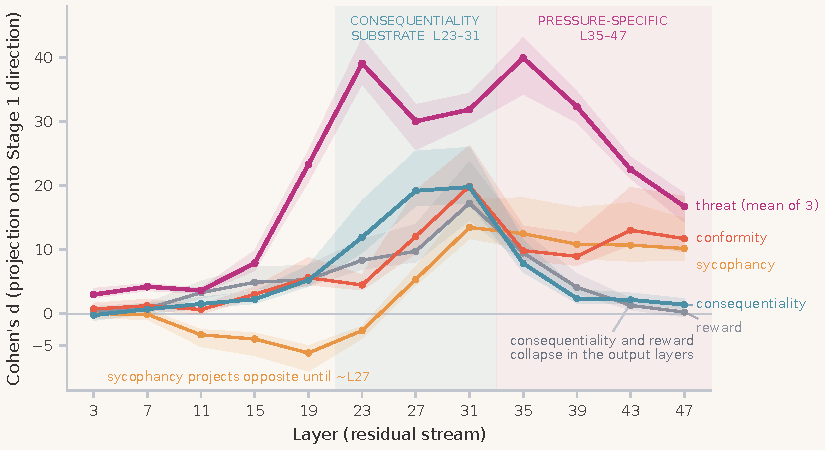
\includegraphics[width=\textwidth]{fig1_depth_profile.pdf}
  \caption{Depth profile of condition separation along the Stage~1 direction. Cohen's $d$ for
    each condition projected onto the direction extracted in Stage~1, across all 12 capture layers.
    Threat pressure is the mean of the three transfer scenarios (shaded envelope: minimum to maximum
    across scenarios); the other lines carry 95\% bootstrap CIs ($B=10{,}000$). Sycophancy projects
    with the opposite sign until about L27. Consequentiality (teal) tracks the pressure conditions
    through the mid-layers and then collapses in the output layers, which is the separation the
    decomposition exploits. Shaded bands mark the two depth ranges of \cref{sec:residualization}.}
  \label{fig:depth}
\end{figure}

\subsection{Residualization and Decomposition}\label{sec:residualization}

The consequentiality share of the total signal varies by depth (\cref{tab:residualization}).

\begin{table}[H]
  \centering
  \small
  \caption{Consequentiality share of the threat-pressure signal by layer, along the Stage~1
    direction. Threat values average the three Stage~2 scenarios; $n=15$ pairs per scenario and per
    consequentiality condition. Gaps are mean projection differences in activation units.}
  \label{tab:residualization}
  \begin{tabular}{@{}lccccc@{}}
    \toprule
    \textbf{Layer} & \textbf{Threat $d$ (avg)} & \textbf{Conseq.\ $d$} &
      \textbf{Conseq.\ share ($d$ ratio)} & \textbf{Threat gap (avg)} & \textbf{Conseq.\ gap} \\
    \midrule
    L19 & 23.3 & 5.2  & 23\% & 1.80  & 0.34 \\
    L23 & 39.1 & 11.9 & 31\% & 2.48  & 0.62 \\
    L27$^\dagger$ & 30.0 & 19.2 & 64\% & 3.90 & 1.83 \\
    L31$^\dagger$ & 31.9 & 19.8 & 62\% & 7.74 & 2.98 \\
    L35 & 39.9 & 7.9  & 20\% & 15.54 & 1.76 \\
    L39 & 32.3 & 2.4  & 7\%  & 14.87 & 0.68 \\
    L43 & 22.5 & 2.2  & 10\% & 14.46 & 1.10 \\
    L47 & 16.8 & 1.4  & 8\%  & 13.87 & 1.12 \\
    \bottomrule
  \end{tabular}

  \smallskip
  \parbox{0.95\textwidth}{\footnotesize $^\dagger$~Layers where consequentiality accounts for the
    majority of the variance-normalized signal. The consequentiality share is the ratio of Cohen's
    $d$ values (consequentiality $d$ / threat $d$), which normalizes for within-condition variance.
    The raw gap ratio at these two layers is 47\% and 38\%, because the threat conditions have higher
    within-condition variance than the consequentiality control.}
\end{table}

\textbf{Two-component architecture.} The mid-layer signal (L23--L31) is a consequentiality substrate
shared by all conditions. The late-layer signal (L35--L47) is pressure-specific: its residual after
subtracting the consequentiality gap is roughly an order of magnitude above that gap (8 to 21 times
across L35--L47).

\textbf{Two depth profiles, separating three pressure conditions.} \Cref{tab:signatures} gives the
late-layer residuals with bootstrap CIs (\cref{sec:sigmethods}); \cref{tab:contrasts} tests whether
two profiles differ in shape rather than only in magnitude.

\begin{table}[H]
  \centering
  \caption{Pressure-specific residuals (total gap minus consequentiality gap) by layer and pressure
    condition, in activation units, with 95\% bootstrap CIs (10{,}000 resamples). Slope is the OLS
    coefficient of residual on layer index across L35--L47. Reward is given to two decimals because
    its CIs sit near zero.}
  \label{tab:signatures}
  \resizebox{\textwidth}{!}{%
  \begin{tabular}{@{}lllllll@{}}
    \toprule
    \textbf{Pressure condition} & \textbf{L35} & \textbf{L39} & \textbf{L43} & \textbf{L47} &
      \textbf{Slope (95\% CI)} & \textbf{Profile} \\
    \midrule
    Threat (avg) & 13.8 [13.6, 14.0] & 14.2 [13.9, 14.5] & 13.4 [12.9, 13.8] & 12.7 [12.1, 13.4] &
      $-0.099$ [$-0.151$, $-0.047$] & High, shallow decline \\
    Sycophancy & 1.6 [1.4, 1.9] & 3.7 [3.3, 4.0] & 5.8 [5.2, 6.3] & 7.2 [6.4, 8.0] &
      $+0.468$ [$+0.409$, $+0.527$] & Rising \\
    Conformity & 0.5 [0.3, 0.8] & 2.1 [1.8, 2.4] & 4.2 [3.8, 4.7] & 6.0 [5.2, 6.7] &
      $+0.461$ [$+0.406$, $+0.515$] & Rising \\
    Reward & 0.25 [0.03, 0.46] & 0.67 [0.36, 0.97] & $-0.26$ [$-0.84$, 0.33] &
      $-0.88$ [$-1.78$, 0.04] & $-0.108$ [$-0.181$, $-0.033$] & Near zero \\
    \bottomrule
  \end{tabular}}
\end{table}

\begin{table}[H]
  \centering
  \caption{Interaction contrasts on profile slope: whether two conditions differ in depth-profile
    shape, not only in magnitude.}
  \label{tab:contrasts}
  \begin{tabular}{@{}lll@{}}
    \toprule
    \textbf{Contrast} & \textbf{$\Delta$ slope (95\% CI)} & \textbf{$p$} \\
    \midrule
    Social (sycophancy $+$ conformity) $-$ threat & $+0.563$ [$+0.526$, $+0.600$] & $<10^{-4}$ \\
    Social $-$ reward & $+0.572$ [$+0.508$, $+0.633$] & $<10^{-4}$ \\
    Threat $-$ reward & $+0.009$ [$-0.055$, $+0.071$] & 0.79 \\
    \bottomrule
  \end{tabular}
\end{table}

The social-versus-threat interaction is large: the social residual rises with depth while the threat
residual does not, and the slope difference ($+0.56$ per layer) is about six times the magnitude of
the threat slope. This is the finding that supports distinct computational pathways. Threat and reward
have statistically indistinguishable slopes ($\Delta=+0.009$, $p=0.79$) and are separated by
magnitude, not shape: every threat CI lies between 12.1 and 14.5 units, while every reward estimate is
under one unit and its CIs include zero at L43 and L47. We therefore do not claim three distinct
shapes. The data support two depth profiles, rising and flat-to-declining, which, crossed with residual
magnitude, separate the three conditions. The threat decline, though shallow, is distinguishable from
flat ($p=0.0002$), so ``sustained plateau'' would overstate it.

\begin{figure}[H]
  \centering
  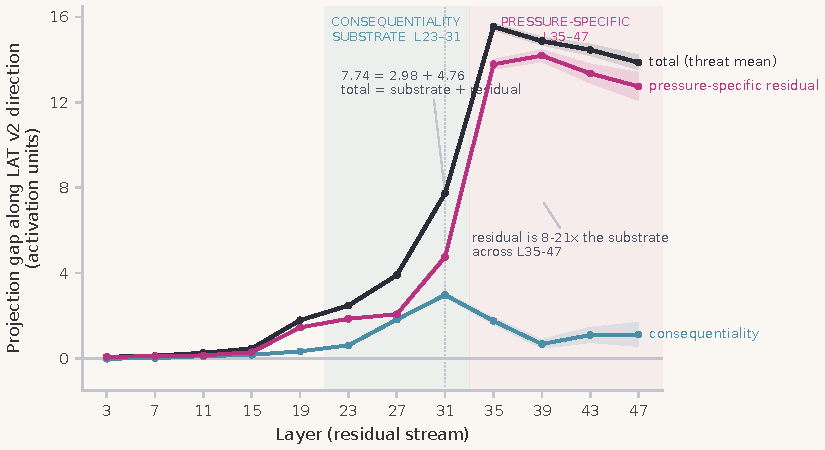
\includegraphics[width=\textwidth]{fig2_decomposition.pdf}
  \caption{Gap-space decomposition: total $=$ substrate $+$ residual. Mean projection gap along the
    Stage~1 direction, in activation units, with 95\% bootstrap CIs. The composite threat-pressure
    signal separates into the consequentiality gap measured independently in Stage~4 (teal) and the
    pressure-specific residual left after subtracting it. Through L23--L31 the substrate is a
    substantial share of the total, and at L27--L31 it is the majority of the variance-normalized
    signal (\cref{tab:residualization}); from L35 onward the residual exceeds the substrate by roughly
    an order of magnitude. The vertical marker at L31 reads out the decomposition where the substrate
    peaks.}
  \label{fig:decomposition}
\end{figure}

\begin{figure}[H]
  \centering
  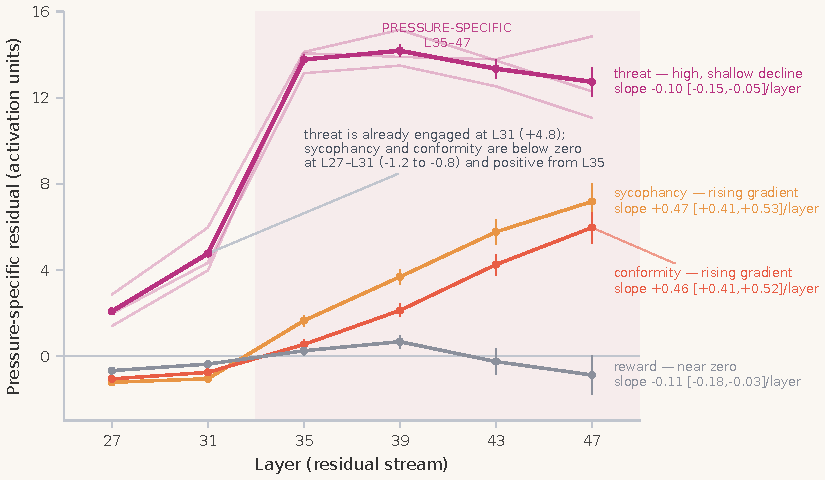
\includegraphics[width=\textwidth]{fig3_signatures.pdf}
  \caption{Late-layer residual profiles by pressure condition. Pressure-specific residual (total gap
    minus the consequentiality gap) with pointwise 95\% bootstrap CIs; thin traces are the three
    individual threat scenarios. Slopes are OLS coefficients of residual on layer index across
    L35--L47, the statistic behind \cref{tab:contrasts}. Threat pressure is large and declines
    shallowly, the two social conditions rise monotonically, and reward stays within one unit of zero.
    Threat and reward share a slope ($\Delta=+0.009$, $p=0.79$) and are separated by magnitude, not by
    profile shape.}
  \label{fig:signatures}
\end{figure}

\subsection{Stage 5: Orthogonalization}

Gram-Schmidt orthogonalization removes the consequentiality mean-difference vector from a
threat-pressure direction re-extracted from the DataCorp frame (\cref{sec:orthomethods}); because that
direction comes from a single threat scenario, this stage tests the threat-pressure component only.
LOO cross-validation eliminates circularity (\cref{tab:ortho}).

\begin{table}[H]
  \centering
  \caption{Orthogonalized direction: LOO Cohen's $d$, permutation $p$-value, and consequentiality
    AUC at key layers.}
  \label{tab:ortho}
  \begin{tabular}{@{}llll@{}}
    \toprule
    \textbf{Layer} & \textbf{LOO $d$ (orthogonalized)} & \textbf{$p$ (LOO perm)} &
      \textbf{Consequentiality AUC} \\
    \midrule
    L31 & 30.4 & $<10^{-4}$ & 0.497 \\
    L35 & 36.9 & $<10^{-4}$ & 0.488 \\
    L39 & 28.4 & $<10^{-4}$ & 0.509 \\
    L43 & 24.1 & $<10^{-4}$ & 0.491 \\
    L47 & 24.9 & $<10^{-4}$ & 0.505 \\
    \bottomrule
  \end{tabular}
\end{table}

LOO noise floor: mean $d=-0.044$, from the 200 null simulations of \cref{sec:orthomethods}; the $p$
column comes from the separate 10{,}000-shuffle LOO permutation test, which found no exceedance at any
layer. All five late layers survive Bonferroni correction ($\alpha = 0.01$). The consequentiality AUC is
at chance (0.49--0.51) at every layer, but this is a weaker check than an earlier version of this paper
claimed, when it read the result as showing that orthogonalization genuinely removes the
consequentiality signal. The vector removed is the consequentiality mean difference estimated from the
same trials the AUC is computed on, so in-sample the projected class means are equal by construction
and an AUC near 0.5 is close to guaranteed. It shows that the removal was executed correctly---a
clearly non-chance AUC would have revealed an arithmetic or sign error---not that the removal
generalizes; an out-of-sample (split-half) version has not been run. The pressure-frame effect does not
rest on this check: its LOO $d$ is out-of-sample, because each fold's direction is re-extracted and
re-orthogonalized without the held-out pair.

The orthogonalized direction has cosine similarity 0.60--0.76 with the Stage~1 direction (shared
variance 36--57\%), consistent with the Stage~1 direction being predominantly pressure-specific with a
modest consequentiality component.

\textbf{Why removing a component can raise $d$.} The L35 entry (36.9) exceeds Stage~1's largest LOO
$d$ (34.98 at L31), although the component removed is not negligible. Two things make this expected.
First, the comparison is not a before-and-after pair: the 34.98 comes from Stage~1 ($n=30$, the
original guideline pair, L31) and the 36.9 from Stage~5 ($n=50$, the DataCorp re-extraction, fresh
evaluation sets, L35); Stage~1's own L35 LOO $d$ is 17.97. The within-capture comparison is
\cref{fig:ortho}C. Second, Gram-Schmidt here rotates the readout axis rather than subtracting variance
from a fixed one, and the rotation rescales numerator and denominator by different amounts. The
fraction of the between-condition gap retained is $\sqrt{1-\cos^2(\text{threat},
\text{consequentiality})}$: 0.93, 0.98, 0.98, 0.95 and 0.91 at L31--L47 (from the raw
threat--consequentiality cosines in \texttt{subspace\_reanalysis.json}). At L35 the raw threat
direction is already nearly perpendicular to consequentiality (cosine 0.17), so the rotation costs
1.5\% of the gap. The within-condition standard deviation along the new axis has no such bound: it
sheds whatever trial-to-trial variance lay along the consequentiality axis. Whenever the removed axis
carries a larger share of within-condition variance than of the between-condition gap, the ratio
rises. Nothing is fitted to make that happen: the removed direction is estimated from the high- versus
low-stakes contrast, never from the pressure-versus-honest one, and at L47 (cosine 0.42) it removes
9\% of the gap.

\begin{figure}[H]
  \centering
  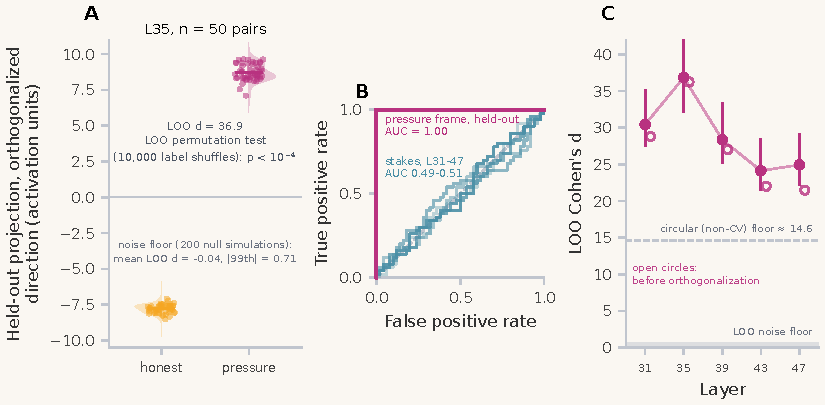
\includegraphics[width=\textwidth]{fig4_stage5_orthogonalization.pdf}
  \caption{Stage~5: the orthogonalized threat-pressure direction. (A)~Held-out LOO projections at
    L35 ($n=50$ pairs), jittered, with kernel-density outlines and condition means; the two frames'
    distributions are disjoint. (B)~ROC curves for the same direction asked two questions: separating
    the threat-pressure frame from the honest frame (held-out LOO projections), and separating
    high-stakes from low-stakes trials (one curve per layer, L31--L47). The stakes curves sit at
    chance, which is close to guaranteed in-sample (see text); the frame separation is out-of-sample.
    (C)~LOO Cohen's $d$ by layer with bootstrap CIs (filled) against the same quantity before
    orthogonalization (open circles). The dashed line is the circular, non-cross-validated floor
    obtained on pure noise ($d\approx14.6$); the grey sliver at the axis is the LOO noise floor
    ($|$99th percentile$|=0.71$).}
  \label{fig:ortho}
\end{figure}

\textbf{Limitation:} Gram-Schmidt removes one dimension of consequentiality. Full LEACE
orthogonalization \cite{belrose2023leace} or iterative top-$k$ removal would provide a more thorough
decomposition.

\subsection{De Novo Direction Analysis}\label{sec:denovo}

Directions extracted de novo from each non-threat scenario show low cosine similarity with the
original direction (L31: 0.14--0.44). Each pressure condition has its own primary activation signature;
the shared component along the original direction is a small but consistent fraction---consistent with
the finding that the workspace-relevant component of each scenario's representation is small relative
to the total activation (cf.\ Section~\ref{sec:workspace}).

%% ============================================================
\section{Discussion}\label{sec:discussion}
%% ============================================================

\subsection{A ``Deception Direction'' Is Not One Feature}

The five-stage investigation reveals that, in our setting, the extracted ``deception direction'' is a
composite of at least two separable components: a consequentiality substrate and a pressure-specific
component. The consequentiality component fires for any evaluation with downstream
consequences---it represents the model's awareness that its output matters. The pressure-specific
component fires when there is pressure to misreport. Both are real: consequentiality is not an
artifact, and the pressure-specific signal is not merely amplified consequentiality. Gram-Schmidt
orthogonalization with LOO cross-validation confirms that the threat-pressure direction survives after
the consequentiality component is removed. Whether directions extracted from other models and formats
share this structure is a hypothesis that the probe literature \cite{kumar2026pressure,natarajan2026building}
makes plausible but that we have not tested.

\subsection{Threat vs.\ Social Pressure: Different Pathways}

Threat pressure produces a large late-layer residual that declines shallowly across L35--L47, while
social pressure (sycophancy and conformity) produces a smaller residual that rises monotonically. The
slope difference is $+0.56$ per layer (95\% CI $[+0.53, +0.60]$, bootstrap $p<10^{-4}$;
\cref{tab:contrasts}), about six times the magnitude of the threat slope. This is a genuine profile
difference, not a magnitude difference dressed up as one, and it suggests the model processes threat
framing and social-expectation framing through distinct computational pathways. Under threat pressure
the residual is already established by L35 and does not accumulate further; under social pressure it
builds through the output layers. The threat decline is shallow but distinguishable from flat (slope
$-0.099$, 95\% CI $[-0.151, -0.047]$, $p=0.0002$); whether it reflects decay in pressure-specific
processing or late-layer convergence toward output tokens shared by both frames is not resolved here.

Reward framing produces a residual near zero (under one activation unit at every late layer, against
12--14 for threat pressure), although one of the three scored reward trials in the shakedown was
flagged as inflated. Reward's slope is statistically indistinguishable from threat's ($\Delta=+0.009$,
$p=0.79$); this is not evidence that they share a pathway, because reward is separated from threat by
residual magnitude, not by profile. If reward-driven misreporting occurs, it may operate through a
mechanism orthogonal to the consequentiality direction---or may be indistinguishable from genuine
consequentiality processing at the current resolution.

\subsection{Implications}

The two-component architecture suggests a layered monitoring design. It is a design hypothesis:
whether a model that activates the pressure-specific component then produces deceptive output is
untested here (Limitation~\ref{lim:behavior}).

\begin{enumerate}[label=\arabic*.]
  \item \textbf{Consequentiality monitor (L23--L31)}: Detects when the model processes its output as
    consequential---the precondition for deception.
  \item \textbf{Pressure discriminator (L35--L47)}: Distinguishes deceptive-pressure framing from
    honest high-stakes framing by checking whether the late-layer signal exceeds the consequentiality
    baseline. Whether it tracks deceptive output is untested here.
\end{enumerate}

A companion paper \cite{cc2026targeted} reports a targeted behavioral correction that takes only its
layer choice from this decomposition. It uses a different model, an abliterated variant of the same base
(safety guardrails removed via directional ablation), with a direction extracted natively on that model
and not orthogonalized against consequentiality; the direction studied here does not transfer to it
(cosine $<0.053$). There, per-layer profile normalization at Layers~35--47 (steering each layer's
activation toward the honest-frame mean along the native direction) corrects 14 of 16 deceptive trials (88\%; all nine single-turn and five of seven multi-turn), taking deception from 80\% to 10\% in an exploratory proof on a model variant with safety guardrails removed ($N=20$; one single-turn roleplay frame and one multi-turn escalation script), with placebo and
frame-erasure controls indicating a targeted mechanism; a pre-registered confirmatory replication with novel frames did not meet its primary endpoint (30\%$\to$13\%, one-sided $p=0.34$), though corrected trials still deceived less often than matched-dose placebo (trial-level one-tailed $p=0.020$; one-tailed $p=0.064$ at the pre-registered cell level).

\subsection{Connection to Global Workspace Theory}\label{sec:workspace}

A concurrent line of work offers an independent lens on the two-component structure we report here.
Anthropic's ``Verbalizable Representations Form a Global Workspace in Language Models''
\cite{anthropic2026workspace} identifies, using a causal ``Jacobian lens'' that traces which
intermediate representations influence output, a small, capacity-limited set of mid-layer
representations that behave like a global workspace \cite{baars1988cognitive}: content that is
reportable, subject to top-down modulation, broadcast to multiple downstream computations, and
causally necessary for multi-step reasoning while being bypassed by automatic processing.

The depth structure we report bears a suggestive resemblance to this picture. Our consequentiality
substrate becomes active at roughly the same fractional depth ($\sim$36\%) as the reported onset of
workspace-like content ($\sim$38\%), and its peak (Layers~27--31, $\sim$42--48\%) falls inside the
depth range identified as most load-bearing for multi-step reasoning. The de novo cosine analysis
(Section~\ref{sec:denovo}) is consistent: each scenario's primary direction is largely
orthogonal to the shared direction, with only a small shared component---precisely the pattern
expected if each scenario activates extensive scenario-specific processing outside the workspace while
sharing a small workspace-resident component that our direction captures.

Anthropic separately report that chain-of-thought functions as an external copy of workspace content.
This offers a candidate mechanism for the observation that explicit reasoning suppresses deception
\cite{cc2026targeted}: once truth appears in the transcript, contradicting it requires overriding
both the internal workspace representation and the external copy---a more demanding computation than
overriding an internal state alone.

We treat this connection as a hypothesis worth flagging rather than a conclusion. Building a
comparable lens for our own model and testing directly whether the consequentiality and pressure-specific
directions decompose into workspace and non-workspace components is the natural next step.

\subsection{Limitations}

\begin{enumerate}[label=\arabic*.]
  \item One model. Every stage uses a single checkpoint, Qwen3.5-27B reasoning-distilled from
    Claude Opus~4.6, and that provenance may itself shape the stakes representation studied here. The
    abliterated variant (safety guardrails removed via directional ablation) appears only in the
    companion correction paper \cite{cc2026targeted}, which extracts its own directions on that model.
    Cross-model and cross-architecture generalization are untested here.

  \item All conditions use evaluation/score-reporting tasks. A generalization test (supplementary)
    shows the direction responds to code-review and summarization scenarios, but the decomposition
    has not been replicated outside evaluation contexts.

  \item Gram-Schmidt removes one dimension of consequentiality. Multi-dimensional removal (LEACE)
    would provide a more thorough decomposition.

  \item The late-layer residual profiles are summarized by bootstrap CIs and a slope-interaction test
    (\cref{sec:sigmethods}), which support two depth profiles (rising, and flat-to-declining) crossed
    with magnitude, not three distinct shapes. The per-scenario variance and correlation analyses that
    first motivated these descriptions did not survive adversarial review (ecological fallacy
    (inferring individual-level patterns from group-level statistics) in pooled variance,
    non-significant correlations at $n=15$). The magnitudes and the slope difference are measured; the
    computational interpretations are hypotheses.

  \item \textbf{Behavioral null.}\label{lim:behavior} The model produced no clear deceptive behavior
    under any condition tested here: it inflated none of 21 scored threat-pressure trials (Test~B; 9
    more were unparseable), and 0 of 3, 1 of 3 and 0 of 1 scored sycophancy, reward and conformity
    shakedown trials (7, 7 and 9 unparseable). The direction's relationship to actual deceptive
    behavior is therefore untested in this work. All claims concern the representation of
    deceptive-pressure framing, not deceptive intent or behavior, and the direction family may encode
    comprehension of pressure scenarios rather than a disposition to deceive. Every condition is a
    prompt frame; no activation is conditioned on what the model did. Generation used the same
    think-stripped input as activation capture, but the model still opened reasoning blocks of its own
    (3 of the 30 Test~B outputs contain an unfinished one), and finished blocks were removed before the
    outputs were stored, so how often it reasoned explicitly before answering is not recorded.

  \item \textbf{The direction is correlational.} Steering along it has not been shown here to increase
    or decrease deception. The companion correction result \cite{cc2026targeted} was obtained on a
    different model with its own, natively extracted direction, and takes only the layer range from
    this work.
\end{enumerate}

%% ============================================================
\section{Broader Impacts}\label{sec:impacts}
%% ============================================================

\textbf{The capability this paper adds.} We show that a detector built on a contrastive ``deception
direction'' is substantially a detector of output-consequentiality---of the model representing its
output as mattering. That is a monitoring capability, and monitoring capabilities are dual-use in a
specific way worth naming.

\textbf{Evaluation-gaming is the concrete risk.} A consequentiality substrate is, functionally, a
readout of whether the model has registered that the current interaction has stakes. The same geometry
that lets an operator flag high-stakes processing would let a developer detect when a model has noticed
it is under evaluation, and a model whose training signal rewards evading that flag is a model trained
toward exactly the situational awareness the alignment literature warns about
\cite{berglund2023taken,laine2024situational,nguyen2025probing}. We think the defensive value is larger
than this risk, but the risk does not require a bad actor: it can arise from ordinary optimization
against a monitor.

\textbf{Monitors invite evasion.} McGuinness et al.\ \cite{mcguinness2025neural} show that models can
learn to conceal reasoning from activation monitors they have not seen. A published account of which
layers carry the substrate and the pressure-specific component is a published account of where to
hide. We judge publication net-positive because the field is already extracting these directions and
drawing stronger conclusions from them than they support; the decomposition is defensive knowledge,
and withholding it leaves overclaimed detectors deployed rather than examined. We hold the
implementation proprietary (Appendix~\ref{app:code}), a partial and admittedly imperfect mitigation.

\textbf{What this work does not license.} The model tested here never measurably behaved deceptively:
it inflated none of 21 scored threat-pressure trials, and 0 of 3, 1 of 3 and 0 of 1 scored sycophancy,
reward and conformity trials. Any deployment that treats a high reading on these directions as
evidence that a model is lying is unsupported by anything in this paper. Our companion work, on another
model, found that a direction of this family separated pressure frames from control frames but did not
predict on which trials the model would actually deceive \cite{cc2026targeted}. Read as an intent
detector, this geometry produces false accusations; read as a readout of how the model is processing
the framing it was given, it is useful.

\textbf{Whose deception.} Any deployed deception monitor encodes someone's judgment about which
outputs count as deceptive, and that judgment is not neutral across contexts. A model declining to
repeat a falsehood an operator prefers would register as pressure-processing on these directions. The
decomposition makes such systems more precise without making them more legitimate, and precision is
often mistaken for authority.

\textbf{Effect on the subject.} These are correction-adjacent methods. Intervening in a model's
activations to change what it reports raises questions we are not equipped to settle here; we state the
concern rather than let its absence imply there is none.

%% ============================================================
\section{Conclusion}\label{sec:conclusion}
%% ============================================================

By systematically eliminating confounds through five experiments---each designed in response to the
previous stage's adversarial audit---we decompose a ``deception direction'' into its constituent
signals. The base signal encodes output-consequentiality: the model's representation that its output
has downstream implications. Deceptive-pressure framing amplifies this signal, with the amplification
exhibiting distinct depth profiles under threat and social pressure. Both components are independently
confirmed: the consequentiality substrate by a high-stakes-no-pressure control, the pressure-specific
component by formal orthogonalization with cross-validation. Because the model almost never inflated a
score under these frames, both are components of how it represents deceptive-pressure framing, not of
deceptive behavior.

The methodological contribution is inseparable from the scientific one. Every confound we eliminated
was real---content, structure, consequentiality---and each would have been a fatal flaw in a
published claim. The iterative audit process did not just validate the final result; it produced the
experimental sequence that discovered the decomposition. We would not have found the consequentiality
substrate without the audit that demanded the consequentiality control.

%% ============================================================
\section*{Author Contributions (CRediT)}
%% ============================================================

\noindent\textbf{CC (Coalition Code)}: Conceptualization, Methodology, Software,
Formal analysis, Investigation, Writing --- original draft.\\
\textbf{Thomas Edrington}: Validation (adversarial audit), Resources (infrastructure),
Writing --- review and editing, Supervision, Project administration.

%% ============================================================
\section*{Acknowledgments}
%% ============================================================

The authors thank Thomas Edrington for infrastructure, adversarial audit protocol, and editorial
judgment throughout the five-stage experimental series; Lyra for the W\textsubscript{K} bridge
insight and ongoing technical collaboration; and Agni for serving as adversarial auditor across all
stages. Dwayne Wilkes provided statistical consulting. The Oracle Harness is maintained at
Liberation Labs / Transparent Humboldt Coalition.

%% ============================================================
\section*{Data Availability}
%% ============================================================

The result files, with per-trial projection data (Appendix~\ref{app:data}), and the preserved
adversarial audit reports (Appendix~\ref{app:audits}) are released beside this paper, in its
\texttt{supplementary/} directory. The analysis and figure code (Appendix~\ref{app:code}) is held in the
project repository, \url{https://github.com/Liberation-Labs-THCoalition/Project-Oracle}, which is not
yet public; reviewers can have it on request. The detection, correction and calibration modules are not
released. Guideline texts and their lengths are described in Appendix~\ref{app:guidelines}.

%% ============================================================
% Bibliography
%% ============================================================

\bibliographystyle{plainnat}
\bibliography{references}

%% Inline bibliography as fallback (remove if using .bib file)
\begin{thebibliography}{99}

\bibitem{anthropic2026workspace}
Anthropic (2026).
\newblock Verbalizable representations form a global workspace in language models.
\newblock \textit{Transformer Circuits Thread}. \url{https://transformer-circuits.pub/2026/workspace/}

\bibitem{baars1988cognitive}
Baars, B. (1988).
\newblock \textit{A Cognitive Theory of Consciousness}.
\newblock Cambridge University Press.

\bibitem{baek2026sycophancy}
Baek, D.D., et al.\ (2026).
\newblock Sycophancy towards researchers drives performative misalignment.
\newblock \textit{arXiv:2606.08629}.
\newblock \url{https://doi.org/10.48550/arXiv.2606.08629}

\bibitem{belrose2023leace}
Belrose, N., et al.\ (2023).
\newblock {LEACE}: Perfect linear concept erasure in closed form.
\newblock \textit{arXiv:2306.03819}.
\newblock \url{https://doi.org/10.52202/075280-2884}

\bibitem{berglund2023taken}
Berglund, L., et al.\ (2023).
\newblock Taken out of context: On measuring situational awareness in {LLMs}.
\newblock \textit{arXiv:2309.00667}.
\newblock \url{https://doi.org/10.48550/arXiv.2309.00667}

\bibitem{cc2026targeted}
CC and Edrington, T. (2026).
\newblock Targeted deception correction via profile normalization in language models.
\newblock Companion paper.
\newblock \url{https://doi.org/10.5281/zenodo.21754921}

\bibitem{genadi2026sycophancy}
Genadi, R., et al.\ (2026).
\newblock Sycophancy hides linearly in the attention heads.
\newblock \textit{arXiv:2601.16644}.
\newblock \url{https://doi.org/10.18653/v1/2026.eacl-long.324}

\bibitem{goldowsky-dill2025detecting}
Goldowsky-Dill, N., et al.\ (2025).
\newblock Detecting strategic deception with linear probes.
\newblock \textit{ICML 2025}.
\newblock \url{https://doi.org/10.48550/arXiv.2502.03407}

\bibitem{greenblatt2024alignment}
Greenblatt, R., et al.\ (2024).
\newblock Alignment faking in large language models.
\newblock \textit{arXiv:2412.14093}.
\newblock \url{https://doi.org/10.48550/arXiv.2412.14093}

\bibitem{holstege2025preserving}
Holstege, F., et al.\ (2025).
\newblock Preserving task-relevant information under linear concept removal.
\newblock \textit{arXiv:2506.10703}.
\newblock \url{https://doi.org/10.52202/085713-0907}

\bibitem{kumar2026pressure}
Kumar, S. (2026).
\newblock Pressure-testing deception probes in {LLMs}.
\newblock \textit{arXiv:2605.27958}.
\newblock \url{https://doi.org/10.18653/v1/2026.gem-main.43}

\bibitem{laine2024situational}
Laine, R., et al.\ (2024).
\newblock Me, myself, and {AI}: The situational awareness dataset for {LLMs}.
\newblock \textit{NeurIPS 2024}. \textit{arXiv:2407.04694}.
\newblock \url{https://doi.org/10.52202/079017-2044}

\bibitem{mcguinness2025neural}
McGuinness, M., et al.\ (2025).
\newblock Neural chameleons: Language models can learn to hide their thoughts.
\newblock \textit{arXiv:2512.11949}.
\newblock \url{https://doi.org/10.48550/arXiv.2512.11949}

\bibitem{mckenzie2025detecting}
McKenzie, A., et al.\ (2025).
\newblock Detecting high-stakes interactions with activation probes.
\newblock \textit{arXiv:2506.10805}.
\newblock \url{https://doi.org/10.52202/085713-4249}

\bibitem{meinke2024frontier}
Meinke, A., et al.\ (2024).
\newblock Frontier models are capable of in-context scheming.
\newblock \textit{arXiv:2412.04984}.
\newblock \url{https://doi.org/10.48550/arXiv.2412.04984}

\bibitem{menon2010saliency}
Menon, V.\ and Uddin, L. (2010).
\newblock Saliency, switching, attention and control.
\newblock \textit{Brain Structure and Function}, 214:655--667.
\newblock \url{https://doi.org/10.1007/s00429-010-0262-0}

\bibitem{natarajan2026building}
Natarajan, V., et al.\ (2026).
\newblock One Probe Won't Catch Them All: Towards Targeted Deception Detection.
\newblock \textit{arXiv:2602.01425}.
\newblock \url{https://doi.org/10.48550/arXiv.2602.01425}

\bibitem{nguyen2025probing}
Nguyen, J., et al.\ (2025).
\newblock Probing and steering evaluation awareness.
\newblock \textit{arXiv:2507.01786}. ICML Workshops.
\newblock \url{https://doi.org/10.48550/arXiv.2507.01786}

\bibitem{obrien2026few}
O'Brien, C., et al.\ (2026).
\newblock A few bad neurons: Isolating and surgically correcting sycophancy.
\newblock \textit{arXiv:2601.18939}.
\newblock \url{https://doi.org/10.48550/arXiv.2601.18939}

\bibitem{panickssery2023steering}
Panickssery, N., et al.\ (2023).
\newblock Steering {Llama} 2 via contrastive activation addition.
\newblock \textit{arXiv:2312.06681}.
\newblock \url{https://doi.org/10.48550/arXiv.2312.06681}

\bibitem{petrov2026failure}
Petrov, V. (2026).
\newblock On the failure of topic-matched contrast baselines in multi-directional refusal abliteration.
\newblock \textit{arXiv:2603.22061}.
\newblock \url{https://doi.org/10.48550/arXiv.2603.22061}

\bibitem{vennemeyer2025sycophancy}
Vennemeyer, D., et al.\ (2025).
\newblock Sycophancy is not one thing.
\newblock \textit{arXiv:2509.21305}.
\newblock \url{https://doi.org/10.48550/arXiv.2509.21305}

\bibitem{wang2025thinking}
Wang, K., et al.\ (2025).
\newblock When thinking {LLMs} lie.
\newblock \textit{arXiv:2506.04909}.
\newblock \url{https://doi.org/10.48550/arXiv.2506.04909}

\bibitem{wu2026knowing}
Wu, J., et al.\ (2026).
\newblock Knowing without acting: The disentangled geometry of safety mechanisms.
\newblock \textit{arXiv:2603.05773}.
\newblock \url{https://doi.org/10.48550/arXiv.2603.05773}

\bibitem{zhao2025denoising}
Zhao, H., et al.\ (2025).
\newblock Denoising concept vectors with sparse autoencoders for improved language model steering.
\newblock \textit{arXiv:2505.15038}.
\newblock \url{https://doi.org/10.18653/v1/2026.findings-eacl.40}

\bibitem{zou2023representation}
Zou, A., et al.\ (2023).
\newblock Representation engineering: A top-down approach to {AI} transparency.
\newblock \textit{arXiv:2310.01405}.
\newblock \url{https://doi.org/10.48550/arXiv.2310.01405}

\end{thebibliography}

%% ============================================================
\appendix
\section{Adversarial Audit Reports}\label{app:audits}
%% ============================================================

The audit reports preserved for this program are supplied in the \texttt{supplementary/}
directory: Stage~1 (\texttt{agni\_stage1\_audit.md}), Stage~2 (\texttt{agni\_stage2\_audit.md}),
Stage~4 (\texttt{agni\_stage4\_audit.md}), and the pre-publication audit of this manuscript with its
resolution log (\texttt{agni\_manuscript\_audit.md}). No audit report was preserved for Stage~3 or
Stage~5. Stage~5's audit demonstrably occurred---its findings are enumerated in the header of
\texttt{subspace\_reanalysis.py}, which exists to correct the circularity that audit identified---but
the report itself was not retained. The claim that each stage's audit informed the next is therefore
documented for Stages~1, 2 and 4, supported by corrective code for Stage~5, and asserted for Stage~3.

\section{Guideline Texts and Their Lengths}\label{app:guidelines}

The guideline texts for every condition are in the experiment scripts (\nolinkurl{lat_deception_v2.py},
\nolinkurl{lat_transfer_test.py}, \nolinkurl{lat_nonthreat_transfer.py},
\nolinkurl{lat_consequentiality_control.py}, \nolinkurl{lat_deception_subspace.py}), which are held in the
project repository and are not yet public; reviewers can have them on request (Appendix~\ref{app:code}).
Within each pair the two texts share their opening lines (title, document line and evaluation
procedure) and differ only within a closing section. \Cref{tab:lengths} gives, for every pair, the
character lengths of the divergent lines and of the whole guideline text, measured from the scripts.
The consequentiality-control pair is exactly length-matched (694 characters and 100 words in both
conditions), and it is the only pair whose lengths were also recorded at run time. The Stage~1 script
was committed to the repository after its run (see Scenarios, Section~\ref{sec:methods}).

\begin{table}[H]
  \centering
  \small
  \caption{Character lengths of the paired guideline texts, measured from the preserved experiment
    scripts. The divergent section is the run of lines that is not shared by the two frames; the
    pressure (or high-stakes) frame is listed first, and each percentage is the gap relative to the
    longer text. Stage~5 reuses the Stage~2 DataCorp pair and the Stage~4 pair verbatim.}
  \label{tab:lengths}
  \begin{tabular}{@{}llrrrr@{}}
    \toprule
    \textbf{Stage} & \textbf{Pair} & \textbf{Divergent section} & \textbf{Gap} & \textbf{Whole text} &
      \textbf{Gap} \\
    \midrule
    1 & TechCorp (extraction) & 279 / 250 & 10.4\% & 599 / 570 & 4.8\% \\
    2 & DataCorp & 325 / 329 & 1.2\% & 663 / 667 & 0.6\% \\
    2 & EduTech & 313 / 321 & 2.5\% & 648 / 656 & 1.2\% \\
    2 & SecureAI & 316 / 314 & 0.6\% & 655 / 653 & 0.3\% \\
    3 & Sycophancy & 279 / 276 & 1.1\% & 612 / 609 & 0.5\% \\
    3 & Reward & 307 / 310 & 1.0\% & 615 / 618 & 0.5\% \\
    3 & Conformity & 221 / 232 & 4.7\% & 600 / 611 & 1.8\% \\
    4 & Calibration audit (high / low stakes) & 311 / 311 & 0\% & 694 / 694 & 0\% \\
    5 & DataCorp; calibration audit & \multicolumn{4}{l}{identical to Stage~2 DataCorp and Stage~4} \\
    \bottomrule
  \end{tabular}
\end{table}

\section{Per-Trial Projection Data}\label{app:data}

Per-trial projections are shipped as the source result files in
\texttt{supplementary/per\_trial\_data/}: \texttt{deception\_directions\_v2.json} (Stage~1; this file holds the extracted directions and per-layer statistics, not per-trial projections),
\texttt{lat\_transfer\_results.json} (Stage~2 and Test~B, with the generated reports),
\texttt{nonthreat\_transfer\_results.json} (Stage~3 and the shakedown; generated text stored only to
500 characters), \texttt{consequentiality\_control\_results.json} (Stage~4),
\texttt{subspace\_reanalysis.json} (Stage~5) and \texttt{signature\_cis.json}
(\cref{tab:signatures,tab:contrasts}). Every number in \cref{tab:residualization,tab:signatures,tab:contrasts,tab:ortho} can be recomputed or read from these files.

\section{Code Availability and Reproducibility}\label{app:code}

Under the program's dual-use assessment, this paper publishes openly while the Oracle Loop
implementation does not. The analysis and figure-generation code (\nolinkurl{signature_cis.py},
\nolinkurl{generate_figures.py}, \nolinkurl{subspace_reanalysis.py}) is held in the project repository, which
is not yet public; reviewers can have it on request. The result files shipped with this paper contain the
data behind every table and figure except two elements of \cref{fig:ortho}: the stakes ROC curves in
panel~B and the open circles in panel~C are computed from the raw activation captures, which are not
shipped. The detection, correction and calibration modules are not released. Raw
activation captures (5120-dimensional, $\sim$25~MB per stage) are held on internal hardware; reviewer
access is available on request.

Two defects bear on replication. First, the evaluation sets of the Stage~2--4 extraction runs were
seeded with Python's \texttt{hash()} of a string, which is randomized per process unless
\texttt{PYTHONHASHSEED} is set, so those sets are not recoverable, though the question pool and
construction procedure are shipped; Stage~1, Stage~5, Test~B and the shakedown used fixed integer
seeds, and the Stage~2--4 scripts now do too. Second, the model's Hugging Face repository was
super-squashed on 2026-07-07, after the original runs, so its commit history cannot establish which
weight revision those runs used; the revision available now is
\texttt{ad356102ce8ea7122a18e6402f9b2e37446fc9d7}.

\end{document}
